\section{Ecuaciones de Movimiento}

Para describir la dinámica del sistema compuesto por tres péndulos físicos, se realizan varias consideraciones iniciales que permiten que tanto el experimento como la deducción de las ecuaciones de movimiento sean lo más naturales y simplificadas posible.

Inicialmente, como se observa en la \cref{fig:esquema_equilibrio}, se tiene el esquema de los péndulos en sus puntos de equilibrio, donde los ejes de rotación están separados por una distancia \( a \), correspondiente a la longitud natural de los muelles.

\begin{figure}[h]
    \centering
    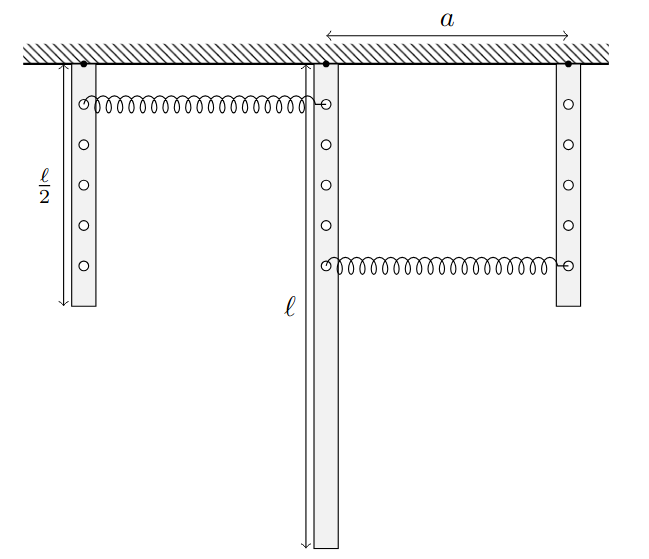
\includegraphics[width=0.8\linewidth]{Figures/Screenshot From 2025-05-25 23-48-28.png}
    \caption{Esquema de los péndulos en equilibrio.}
    \label{fig:esquema_equilibrio}
\end{figure}

La forma empleada para obtener las ecuaciones de movimiento del sistema es mediante una sumatoria de torques, considerando tanto el generado por los resortes como el producido por la fuerza gravitacional.

Es necesario, entonces, encontrar una expresión para el torque gravitacional en función de cualquier ángulo \(\theta_i\), así como una expresión para las distancias del tipo \(x_0 + \Delta x\), que representan la elongación de los resortes en función de los ángulos \(\theta_i\) y \(\theta_{i\pm 1}\).

Las barras se enumeran de izquierda a derecha como 1, 2 y 3, según se muestra en la \cref{fig:enumeracion_barras}.

\begin{figure}[htbp!]
    \centering
    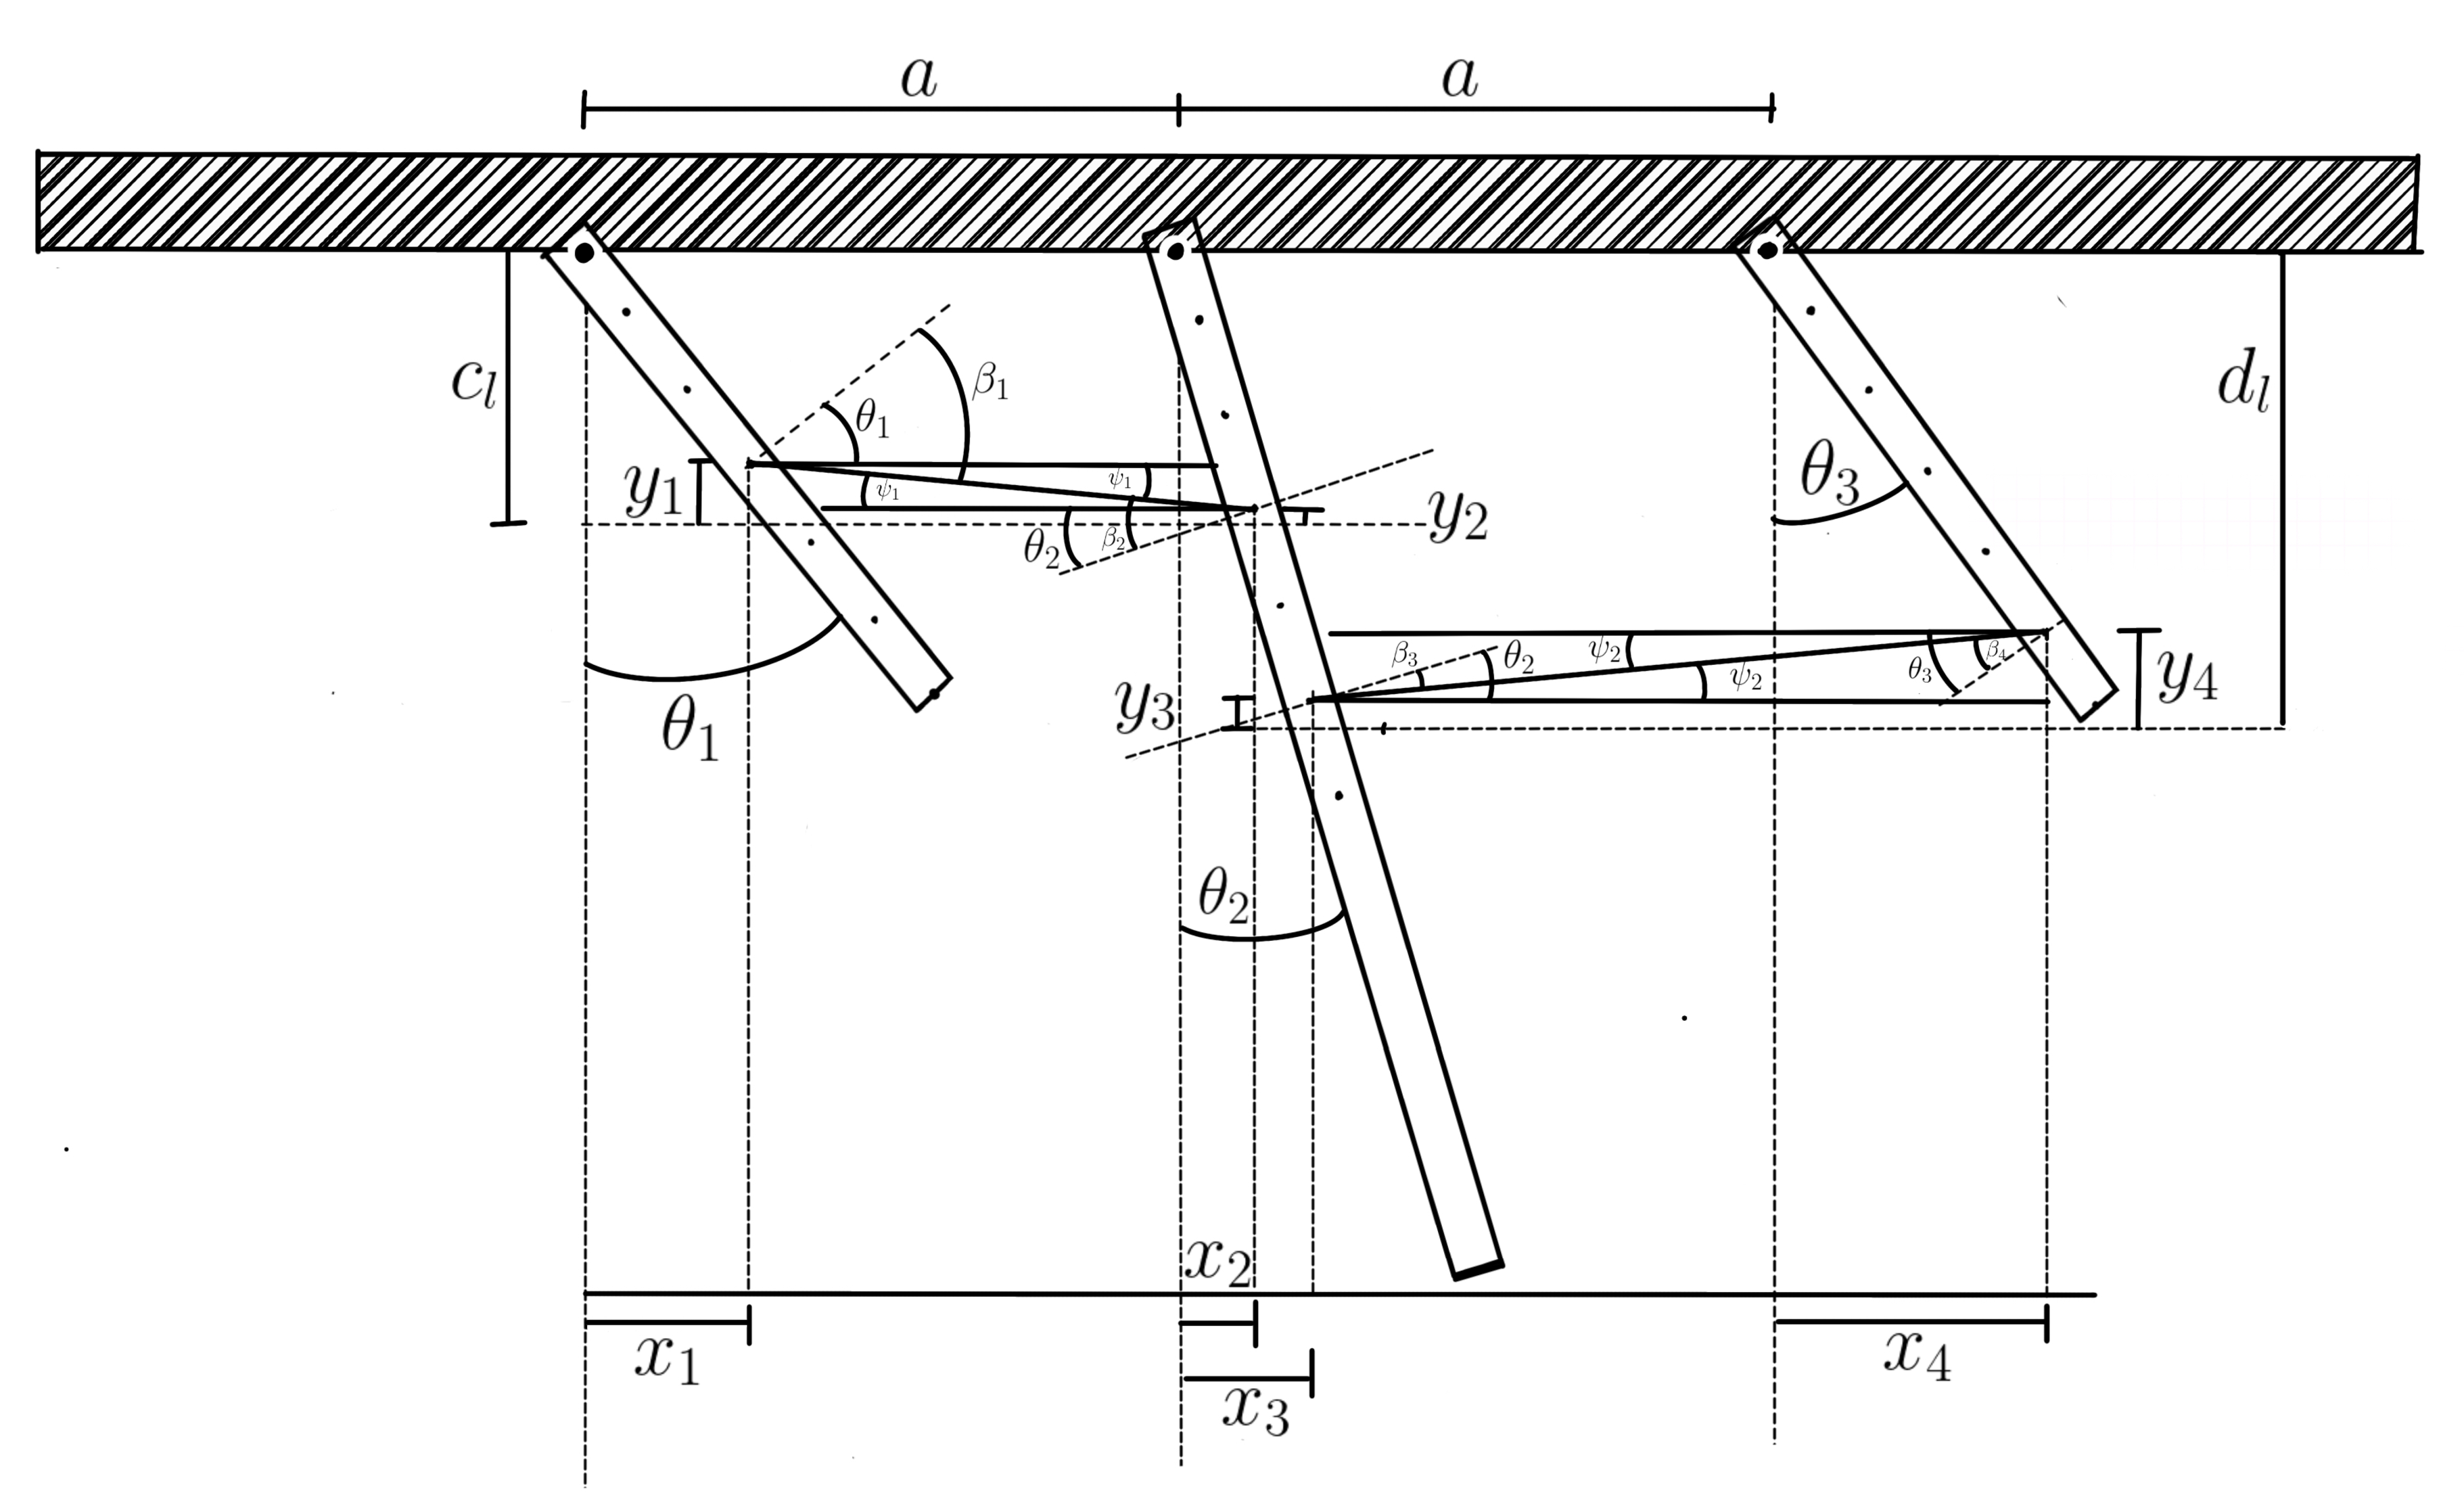
\includegraphics[width=0.8\linewidth]{Figures/Ilustración_sin_título 4.pdf}
    \caption{Numeración de las barras de izquierda a derecha.}
    \label{fig:enumeracion_barras}
\end{figure}

Al desplazar del equilibrio las barras 1 y 2, se observa que la tangente de ambas se desvía del eje horizontal un ángulo \(\theta_i\). Esto permite construir un triángulo rectángulo con las componentes \(x_i\) e \(y_i\) de la posición del punto de aplicación de la fuerza elástica para cada barra, generalizada a cualquier fracción de la longitud \(l\), como se muestra en la \cref{fig:triangulo_posicion}.

\begin{figure}[htbp!]
    \centering
    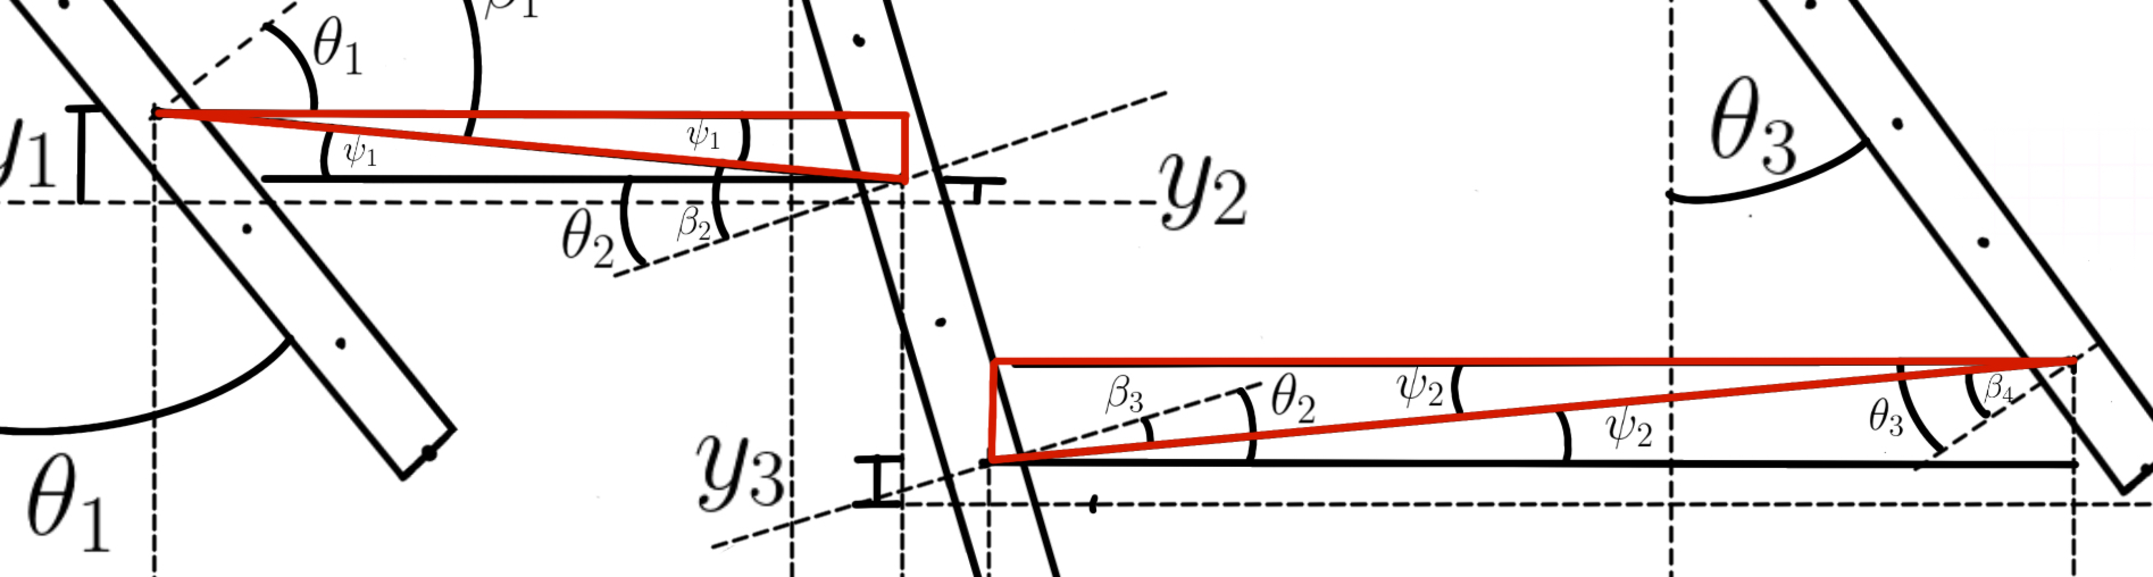
\includegraphics[width=0.8\linewidth]{Figures/Ilustración_sin_título 5.pdf}
    \caption{Construcción geométrica para determinar la posición del punto de aplicación de la fuerza.}
    \label{fig:triangulo_posicion}
\end{figure}

Las coordenadas \(x_k\) e \(y_k\) con \(i = 1, 2\) están definidas como:

\begin{align}
x_k &= c l \sin(\theta_{k}) \\
y_k &= c l \cos(\theta_{k})
\end{align}

El triángulo resultante está definido por un ángulo \(\psi_1\), que cumple la relación \(\beta_1 + \psi_1 = \theta_1\), donde \(\beta_1\) corresponde al ángulo entre la tangente de la barra 1 y la línea recta que conecta los puntos de aplicación. A partir de este triángulo se obtiene la expresión para la elongación del resorte entre las barras 1 y 2:

\begin{equation}
x_{01} + \Delta x_{1} = \sqrt{(y_2 - y_1)^2 + (a + x_2 - x_1)^2}
\end{equation}

Y el ángulo \(\psi_1\) está dado por:

\begin{equation}
\psi_1 = \tan^{-1}\left( \frac{y_2 - y_1}{a - x_1 + x_2} \right)
\end{equation}

De forma análoga, para las barras 2 y 3 se utiliza el punto de aplicación \(dl\), resultando en:

\begin{align}
\psi_2 &= \tan^{-1} \left( \frac{y_4 - y_3}{a - x_3 + x_4} \right), \\
x_{02} + \Delta x_{2} &= \sqrt{(y_4 - y_3)^2 + (a + x_4 - x_3)^2}
\end{align}

Donde para \(j = 3, 4\), \(x_j\) y \(y_j\) son:

\begin{align}
x_j &= d l \sin(\theta_{j}) \\
y_j &= d l \cos(\theta_{j})
\end{align}

El torque gravitacional sobre cada barra está dado por:

\begin{equation}
\tau_{g_i} = \sin(\theta_i) \, y_{\text{cm}_i} \, m_i \, g
\end{equation}

Donde \(y_{\text{cm}_i}\) es la posición del centro de masa de la barra \(i\).

Para los torques elásticos, se deben considerar los ángulos \(\beta_i\), definidos como:

\begin{align}
\beta_1 + \psi_1 &= \theta_1, & \beta_2 + \psi_1 &= \theta_2, \\
\beta_2 + \psi_2 &= \theta_2, & \beta_4 + \psi_2 &= \theta_3
\end{align}

Debido a las distintas posiciones de aplicación entre los pares de barras, aparecen cuatro ángulos \(\beta_i\), donde los índices 2 y 3 están relacionados con la barra central.

La sumatoria de torques, considerando sentido antihorario como positivo, da lugar a:

\begin{align*}
\sum \tau_{m_1} &= \cos(\beta_1) \, c \, l \, k_1 (\Delta x_1) - \sin(\theta_1) \, y_{\text{cm}_1} \, m_1 g = I_1 \, \ddot{\theta}_1, \\
\sum \tau_{m_2} &= \cos(\beta_3) \, d \, l \, k_2 (\Delta x_2) - \cos(\beta_2) \, c \, l \, k_1 (\Delta x_1) - \sin(\theta_2) \, y_{\text{cm}_2} \, m_2 g = I_2 \, \ddot{\theta}_2, \\
\sum \tau_{m_3} &= -\cos(\beta_2) \, d \, l \, k_2 (\Delta x_2) + \sin(\theta_3) \, y_{\text{cm}_3} \, m_3 g = I_3 \, \ddot{\theta}_3
\end{align*}

\subsection*{Aproximaciones para ángulos pequeños}

Con el fin de encontrar una solución analítica aproximada que permita calcular las frecuencias naturales del sistema, se aplican las siguientes aproximaciones:

\begin{align*}
    \sin(\theta) &\approx \theta, \\
    \cos(\theta) &\approx 1, \\
    \tan(\theta) &\approx \theta
\end{align*}

Aplicando estas aproximaciones, las coordenadas se convierten en:

\begin{align*}
x_1 &= c l \theta_1, & x_2 &= c l \theta_2 \\
x_3 &= d l \theta_2, & x_4 &= d l \theta_3 \\
y_1 &= c l, & y_2 &= c l \\
y_3 &= d l, & y_4 &= d l
\end{align*}

Si se cumple que \(x_{01} = x_{02} = a\), las elongaciones de los resortes se simplifican a:

\begin{align*}
\Delta x_1 &= cl(\theta_2 - \theta_1), & \Delta x_2 &= dl(\theta_3 - \theta_2)
\end{align*}

Además, si se asume que \(\tan(\psi_i) \approx \psi_i \approx 0\), entonces \(\beta_i \approx \theta_i\), lo que simplifica la sumatoria de torques a:

\begin{align*}
\sum \tau_{m_1} &= cl k_1 (cl(\theta_2 - \theta_1)) - \theta_1 y_{\text{cm}1} m_1 g = I_1 \ddot{\theta}_1, \\
\sum \tau_{m_2} &= dl k_2 (dl(\theta_3 - \theta_2)) - cl k_1 (cl(\theta_2 - \theta_1)) - \theta_2 y_{\text{cm}_2} m_2 g = I_2 \ddot{\theta}_2, \\
\sum \tau_{m_3} &= dl k_2 (dl(\theta_3 - \theta_2)) + \theta_3  y_{\text{cm}_3} m_3 g = I_3 \ddot{\theta}_3
\end{align*}

Finalmente, el sistema de ecuaciones diferenciales queda:

\begin{equation}
\begin{aligned}
\ddot{\theta}_1 =\; & \theta_1 \left( \frac{(cl)^2 k_{1} - y_{\text{cm}_1} m_1 g}{I_1} \right) + \theta_2 \left( -\frac{k_1 (cl)^2}{I_1} \right) \\
\ddot{\theta}_2 =\; & \theta_1 \left( \frac{k_1 (cl)^2}{I_2} \right) + \theta_2 \left( -\frac{k_1 (cl)^2}{I_2} + \frac{k_2 (dl)^2}{I_2} + \frac{y_{\text{cm}_2} m_2 g}{I_2} \right) + \theta_3 \left( \frac{k_2 (dl)^2}{I_2} \right) \\
\ddot{\theta}_3 =\; & \theta_2 \left( \frac{k_2 (dl)^2}{I_3} \right) + \theta_3 \left( -\frac{k_2 (dl)^2}{I_3} - \frac{y_{\text{cm}_3} m_3 g}{I_3} \right)
\end{aligned}
\end{equation}

\section{Metodología Experimental}

El desarrollo metodológico se divide en varias etapas clave que incluyen el diseño y construcción del montaje, caracterización de sus componentes y adquisición de datos mediante sensores angulares.

\subsection*{Construcción del Montaje}

Para la construcción del sistema se utilizaron tres barras metálicas de alta densidad. Las barras laterales tienen una longitud $l/2 = (\qty{28.0(1)}{\centi\metre}$, mientras que la barra central tiene longitud $l = (\qty{56.0(1)}{\centi\metre}$. Las masas y centros de masa de cada barra fueron determinadas experimentalmente y se resumen en el \cref{tab:parametros}.

\begin{table}[htbp!]
    \centering
    \caption{Parámetros físicos de las barras empleadas.}
    \label{tab:parametros}
    \begin{tabular}{c c c}
        \toprule
        Péndulo ($i$) & $y_{\text{cm},i}$ [cm] & $m_i$ [g] \\
        \midrule
        1 & 14.2 & 600.8 \\
        2 & 28.0 & 1216.3 \\
        3 & 14.0 & 601.8 \\
        \bottomrule
    \end{tabular}
\end{table}

Las barras fueron perforadas para permitir distintos puntos de acople de resortes. La \cref{fig:barras} muestra las barras listas para el montaje.

\begin{figure}[htbp!]
    \centering
    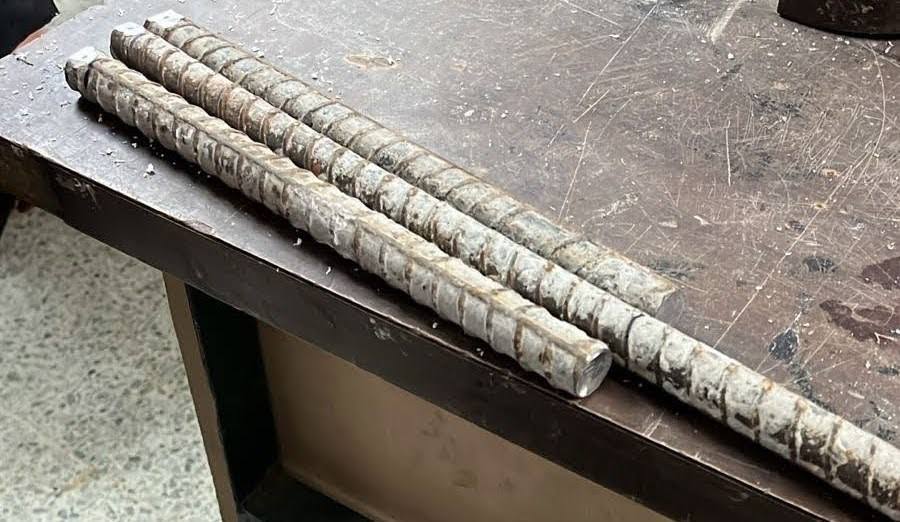
\includegraphics[width=0.6\linewidth]{Figures/metal-bars.jpeg}
    \caption{Barras metálicas preparadas para el montaje de los péndulos.}
    \label{fig:barras}
\end{figure}

\subsection*{Medición de la Constante Elástica}

La constante elástica de los resortes fue determinada mediante la aplicación de masas conocidas y el registro de su desplazamiento. Utilizando una regresión lineal, se obtuvieron los siguientes valores:

\begin{itemize}
    \item $k_1 = \qty{3.04(4)}{\N\per\m}$
    \item $k_2 = \qty{3.32(6)}{\N\per\m}$
\end{itemize}

\begin{figure}[htbp!]
    \centering
    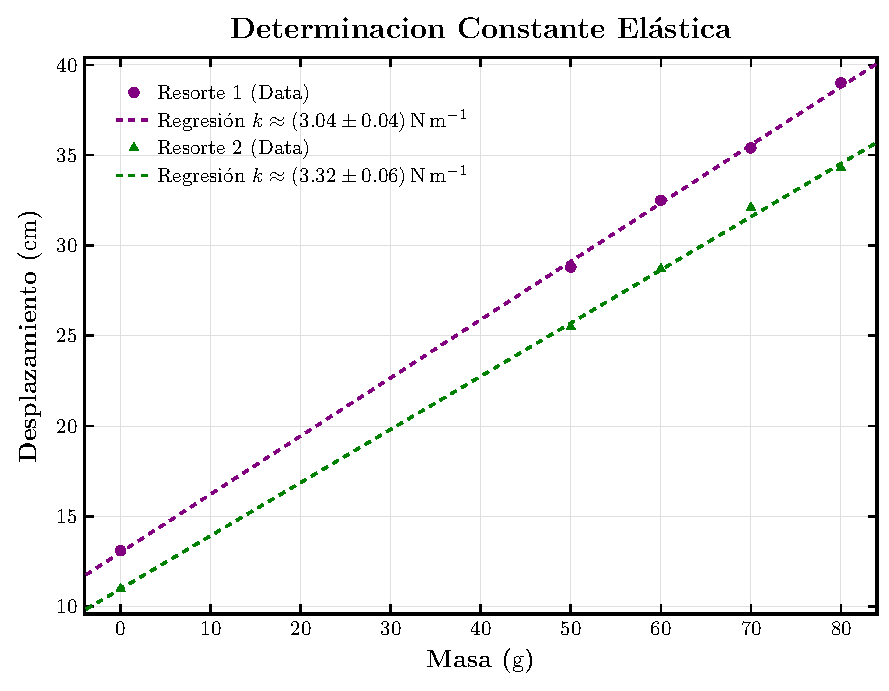
\includegraphics[width=0.75\linewidth]{Figures/springs-plot.pdf}
    \caption{Determinación de la constante elástica mediante regresión lineal.}
    \label{fig:regresion}
\end{figure}

\subsection*{Integración del Sistema de Medición}

Para registrar los desplazamientos angulares $\theta_i(t)$, se integraron sensores angulares rotacionales Cassy en cada punto de pivote de los péndulos. Las barras fueron fijadas a las ruedas del sensor utilizando alambre dulce.

\begin{figure}[htbp!]
    \centering
    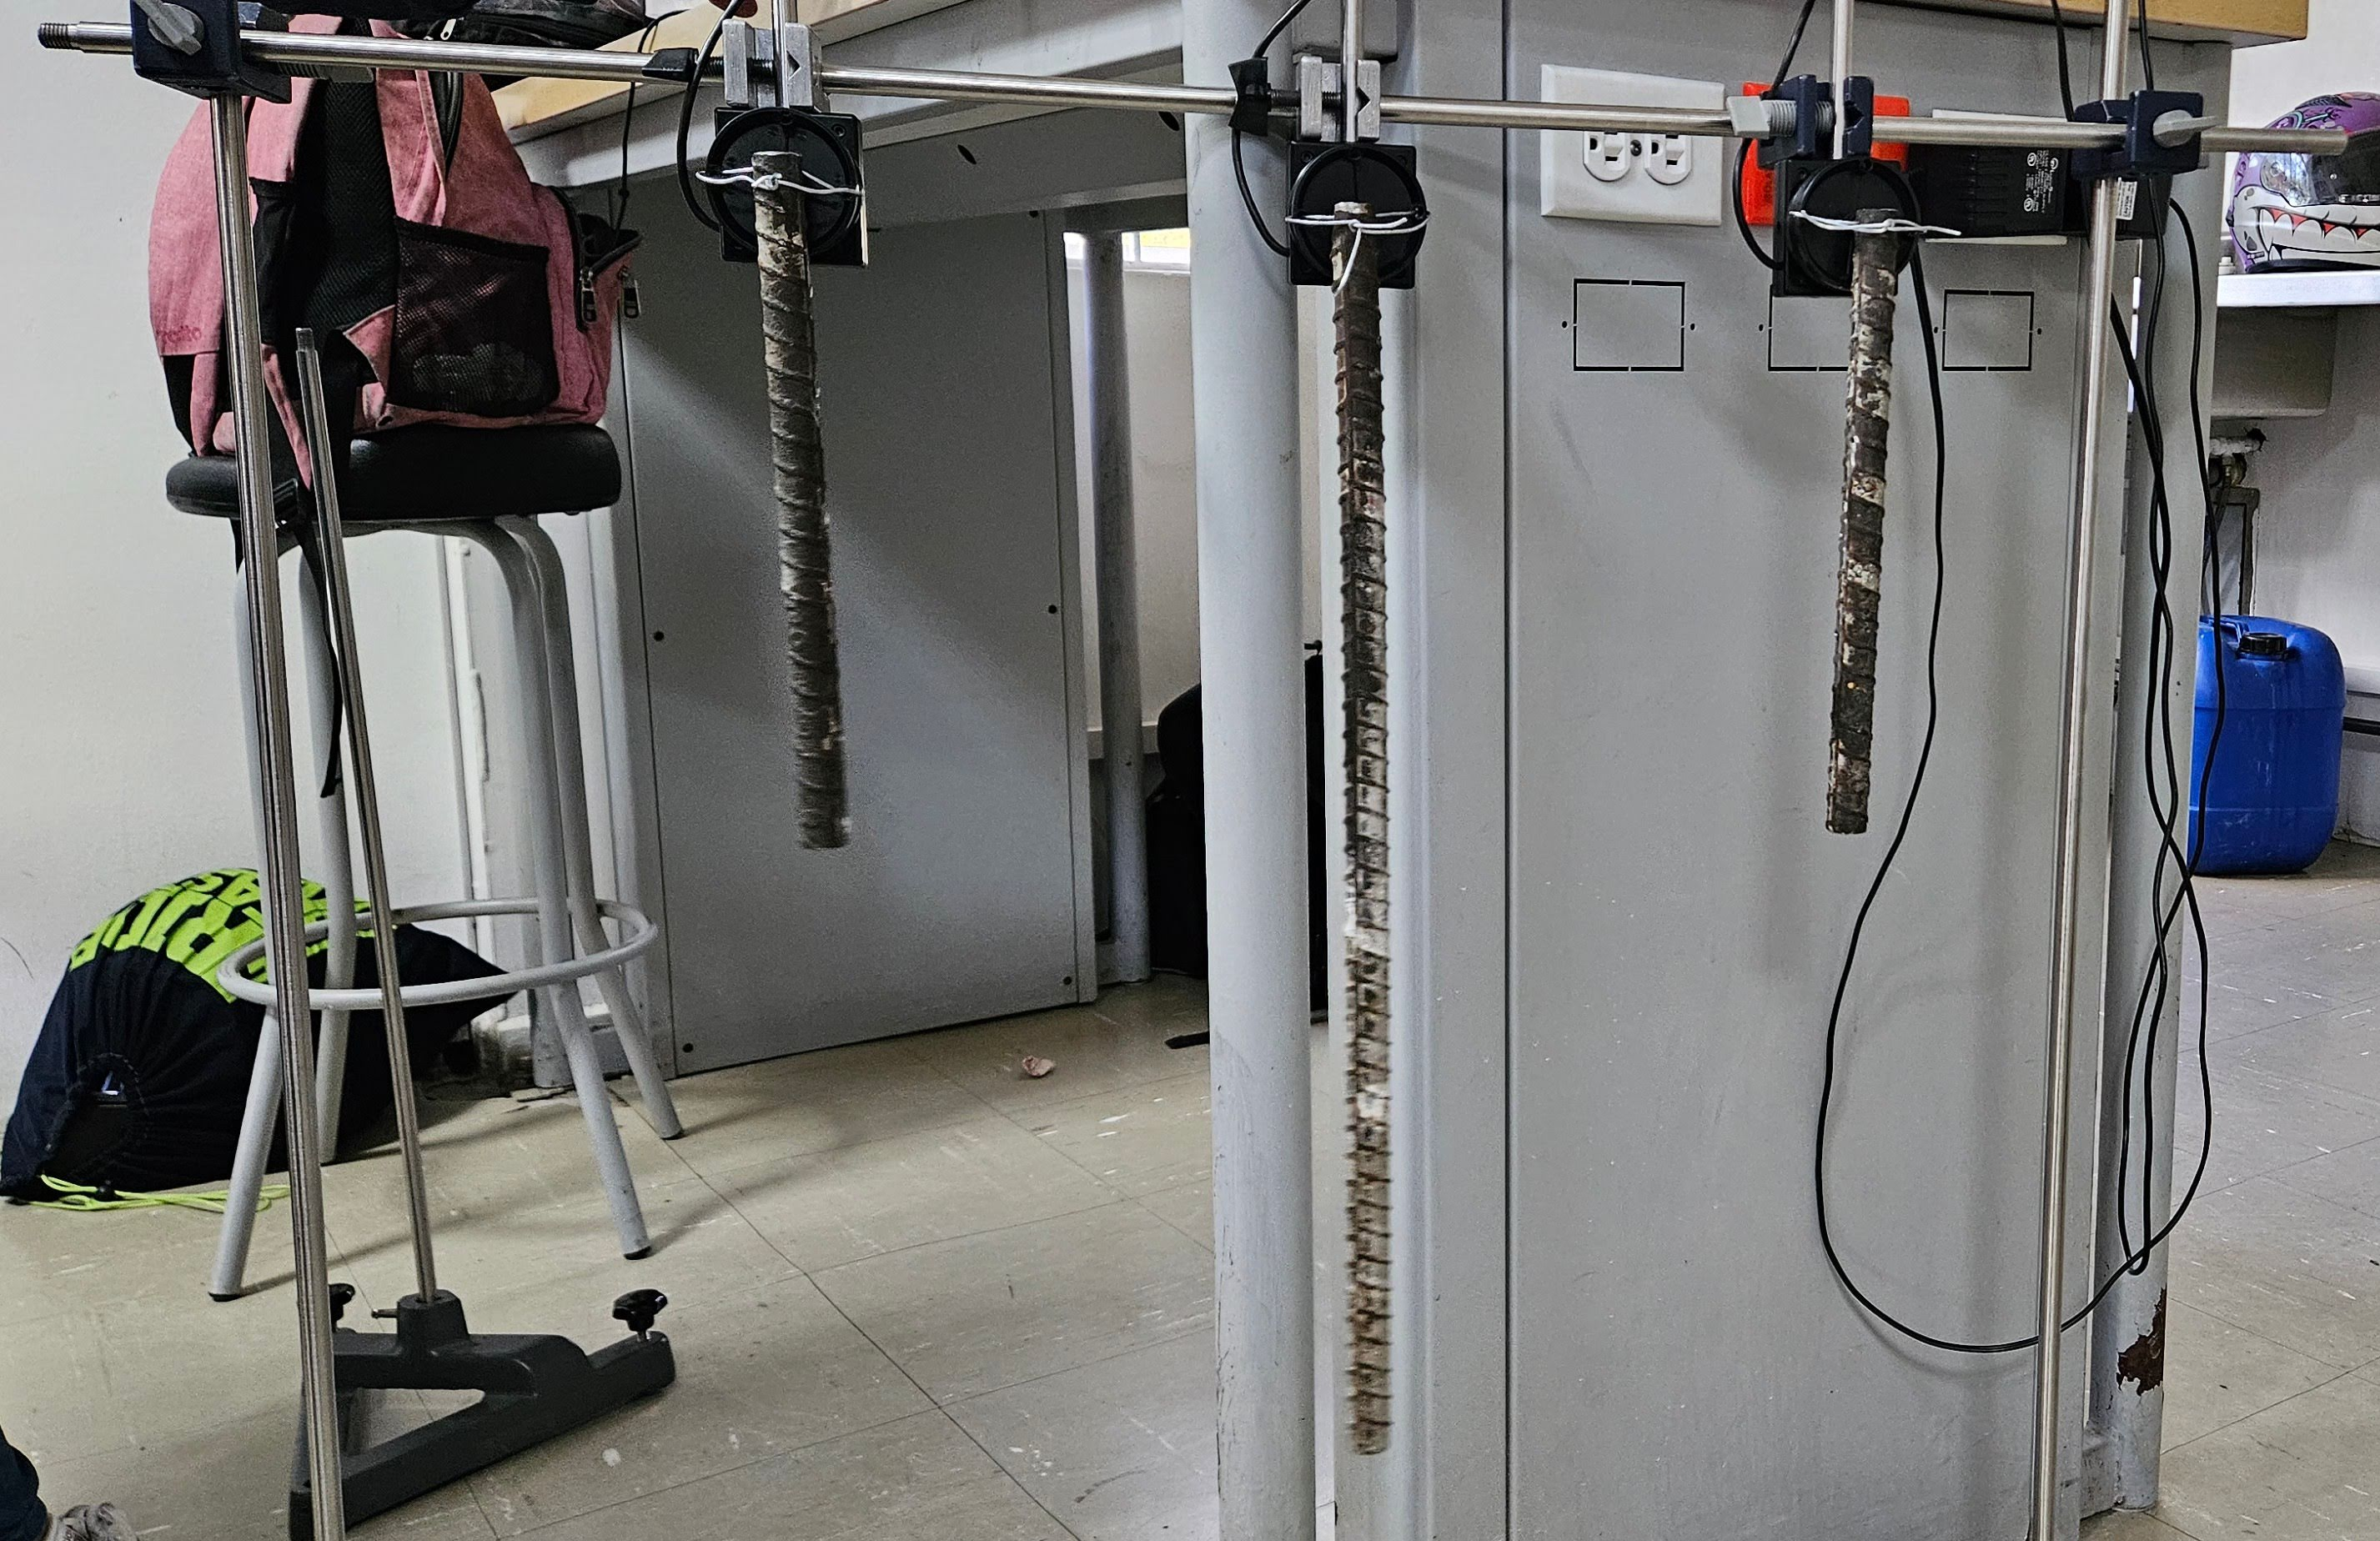
\includegraphics[width=0.75\textwidth]{Figures/set-up.jpeg}
    \caption{Montaje experimental completo con sensores Cassy.}
    \label{fig:montaje}
\end{figure}

\subsection{Toma de Datos}

Se realizaron experimentos bajo cinco configuraciones distintas de acoplamiento (ver \cref{fig:configuraciones}) y tres tipos de condiciones iniciales:

\begin{itemize}
    \item (001): Desplazamiento solo del péndulo 3.
    \item (010): Desplazamiento solo del péndulo 2.
    \item (101): Desplazamiento simétrico de los péndulos 1 y 3.
\end{itemize}

Cada configuración fue registrada durante aproximadamente 30 segundos para capturar múltiples oscilaciones.
Los datos fueron almacenados digitalmente para su posterior análisis y comparación con los resultados teóricos de los modos normales de oscilación.
